\documentclass[11pt]{article}
\usepackage[margin=0.9in]{geometry}
\input{glyphtounicode}
\pdfgentounicode=1
\usepackage{amsmath,booktabs,graphicx}
\usepackage[colorlinks=true,urlcolor=blue,linkcolor=black,citecolor=black]{hyperref}

\setlength{\parindent}{0pt}
\setlength{\parskip}{0.45em}
\title{Conditional Acceptance Calibration for Dynamic Medusa Decoding}
\author{ECE 285 project team\\Ada Qi, Alexander Tung, and Zhuoting Yang\\University of California San Diego}
\date{November 2026}
\begin{document}
\maketitle
\begin{abstract}
The project tests whether conditioning each Medusa head's draft probability on a matching parent improves tree selection at a fixed verification budget. We collected 17,882 complete-horizon states on a frozen Vicuna-7B model, trained and tuned on disjoint AlpacaEval prompts, and replayed five policies on 4,280 states from all 80 MT-Bench first turns. Conditional counts improved the fixed tree at every budget, gaining 0.019 to 0.044 accepted tokens per state. Conditional logistic regression changed acceptance by $-0.0014$ to $+0.0042$ tokens relative to the dynamic probability product. Every paired prompt-bootstrap interval for that contrast included zero. On an eight-question GPU panel, all five trees reproduced greedy outputs at both measured budgets. Their throughput ranged from 0.776 to 0.968 times that of cached greedy. The fixed-tree acceptance gain did not yield an end-to-end speedup on this implementation.


\end{abstract}
\section{Which branches should a verifier check?}
Medusa predicts several future tokens from one hidden state. A verifier evaluates a tree of candidate continuations in parallel and commits its longest matching prefix. Each extra draft node consumes verification capacity. With a fixed capacity, the choice between a likely sibling and a deeper continuation therefore affects how many tokens a round can commit. We study that choice on a frozen Vicuna-7B Medusa-1 checkpoint. Only the rule for scoring branches changes.

Medusa uses head accuracy to construct a fixed tree \cite{medusa}. Dynamic tree attention permits a different tree at each state \cite{plus}. Classifier-based tree construction can also use features beyond a product of token probabilities \cite{direct}. To isolate the effect of scoring, our implementation uses the same five frozen heads, ten candidate ranks per head, best-first tree builder, and draft-node budgets for every policy. The direct classifier is a matched-budget adaptation inspired by C2T.
\section{Scoring and selecting paths}
At a state $x$, let $S_v$ be the event that the rank path $v=(r_1,\ldots,r_d)$ matches the next $d$ draft targets following the backbone token. Acceptance of a child entails acceptance of its parent. The chain rule gives
\[
 P(S_v\mid x)=\prod_{i=1}^{d}P(S_{v_{1:i}}\mid S_{v_{1:i-1}},x).
\]
The first parent is always accepted. The expected token count for a prefix-closed tree $T$ is
$1+\sum_{v\in T}P(S_v\mid x)$ by linearity of expectation. The one counts the backbone token. With monotone scores, best-first expansion selects the highest-scoring feasible frontier node at each step. Every hidden descendant scores at most as high as its frontier ancestor. Induction therefore gives a maximum-score prefix-closed set of $B$ nodes. Maximizing actual expected acceptance additionally requires accurate ordering of path probabilities.

\textbf{Fixed policies.} The marginal baseline multiplies per-head rank hit rates from training. The count estimator fits a conditional hit rate among states in which the parent matched. It groups examples by depth, preceding rank and child rank, and shrinks sparse cells toward the marginal baseline. Each estimator yields one tree per budget.

\textbf{Dynamic policies.} MEDUSA+ multiplies current head probabilities along the path. Conditional logistic regression fits the probability of a child hit on accepted-parent examples and multiplies its fitted factors. The direct logistic classifier predicts the whole-path label on a candidate pool and caps each child score at its parent's score. Both logistic methods use the repository's grouped rank and confidence features. The learned scores can change the tree at each state.
\section{Experimental design}
\textbf{Data and model.} The frozen model was FasterDecoding/medusa-vicuna-7b-v1.3 on one 16-GiB RTX 3080 Ti Laptop GPU. The loader quantized the backbone to NF4 from FP16 and promoted floating-point execution and the five prediction heads to FP32, with TF32 disabled. PyTorch reported 6.93 GiB of allocated GPU tensors after loading. Peak allocation during the seven instrumented diagnostic prompts ranged from 9.51 to 9.58 GiB. All policies shared the same weights, top ten candidates per head and 64-token generation cap. We used the original AlpacaEval split and MT-Bench first turns. Training prompt 801 duplicated MT-Bench question 81 verbatim. Removing the training copy before fitting left 199 training, 50 validation and 80 test inputs. A Unicode-, case- and whitespace-normalized text check found no duplicates among the remaining inputs.

\textbf{Reference trajectory.} At each ordinary cached forward, we recorded the backbone's greedy choice, its probability, and the ranked token IDs and probabilities from the five heads. The next backbone token became the input to the next forward. For head $j$ at state $t$, the label is the rank of the $j$th token after the backbone choice, or a miss if that token falls outside the top ten. Thus the label and candidates refer to one recorded trajectory. This avoids deriving features from a separate teacher-forced execution. An independent audit reconstructs every stored label directly from the ranked candidates and generated IDs. Live tree verification is checked separately.

Training yielded 10,854 complete five-head horizons on 196 prompts. Validation yielded 2,748 on 49 prompts. Three training answers and one validation answer reached EOS before a full horizon and supplied zero labeled states. The coverage manifest retains all four. Only positions with all five future targets enter replay. The endpoint therefore describes interior states of bounded generations.

\textbf{Model selection.} The integrated calibration notebook tunes count smoothing and logistic regularization and rank cap on the validation prompts. It compares three candidate-pool constructions for the direct classifier by validation acceptance at $B=63$. The common calibration pool uses MEDUSA+ to select 64 candidate paths per sampled state (up to 4,000 states per split). Brier score averages squared path-probability errors. Expected calibration error (ECE) uses 15 fixed-width probability bins. A grouped feature ablation refits the conditional classifier with each feature group omitted. The frozen notebook fixes the seed and comparison rules before the evaluation results are used.

\textbf{Endpoints.} Replay scores all five trees at each eligible evaluation state and weights states equally. We use 2,000 paired prompt-bootstrap resamples for differences, retaining all states from each sampled prompt. The fixed contrast uses the marginal tree as its baseline. The dynamic contrast uses MEDUSA+. These are per-budget intervals. The analysis treats the family of budget comparisons as exploratory.

\textbf{Live verification and timing.} We fixed an eight-question panel before fitting by selecting the first MT-Bench question from each category, with a separate writing warmup. For budgets 16 and 63 we check cached-reference token IDs, final output IDs, round prefixes, full candidate ranks and selected-node accept/reject decisions. A separate timing pass runs the five policies and cached greedy in seeded, randomized order within prompts. Throughput divides total generated tokens by total measured time, including prefill and generation. Model loading, tokenization, cache allocation and fixed-tree buffer setup lie outside the timer. A separate synchronized run profiles tree overhead on the first measured prompt.

\section{Results}
\textbf{Do heads succeed together?} On 13,602 training and validation states, the marginal product predicted a 14.30\% hit rate for the path taking the top rank in heads one and two. The observed rate was 19.66\% (2,674 hits), or 1.37 times the product estimate. The second head's marginal top-rank accuracy was 28.39\%. Conditional on a first-head top-rank hit, it reached 39.03\% across 6,852 surviving prefixes. The analogous third-head rates were 17.96\% and 37.55\%. The fifth head reached 47.41\% conditional accuracy, but only 424 prefixes survived to that comparison. The dependence is strongest on some paths and leaves fewer examples for estimating deeper factors.


\subsection{Matched-budget replay on MT-Bench}
Each column below gives mean accepted tokens per complete-horizon state at the indicated number of draft nodes. The two calibration measures use one common path pool across budgets. All 80 evaluation questions contributed, with a median of 59 complete states per question and a range of 1 to 59.
\begin{center}
\begin{tabular}{lrrrrrrr}
\toprule
Policy & 8 & 16 & 32 & 63 & 96 & Brier & ECE\\
\midrule
Fixed marginal & 2.106 & 2.314 & 2.486 & 2.634 & 2.704 & 0.02126 & 0.00643\\
Fixed conditional & 2.150 & 2.342 & 2.516 & 2.653 & 2.725 & 0.02112 & 0.00441\\
MEDUSA+ & 2.268 & 2.452 & 2.604 & 2.726 & 2.792 & 0.01839 & 0.00135\\
Direct classifier & 2.269 & 2.455 & 2.605 & 2.730 & 2.791 & 0.01842 & 0.00172\\
Dynamic conditional & 2.268 & 2.451 & 2.607 & 2.731 & 2.794 & 0.01845 & 0.00125\\
\bottomrule
\end{tabular}
\end{center}


The conditional count table beat the marginal fixed tree at all five budgets. Its largest absolute gain occurred at $B=8$, where acceptance rose from 2.106 to 2.150 tokens per state (a 2.10\% relative gain). At the native-sized budget of 63, the fixed gain was $+0.0192$ (95\% paired interval $[0.0063,0.0341]$). MEDUSA+ still had higher acceptance than either fixed tree at every budget. At $B=63$, conditioning the dynamic logistic model changed acceptance from 2.7264 to 2.7306 ($+0.0042$, interval $[-0.0009,0.0090]$). The direct classifier reached 2.7299. These small differences leave the ordering of the dynamic methods uncertain.

\begin{figure}[htbp]
\centering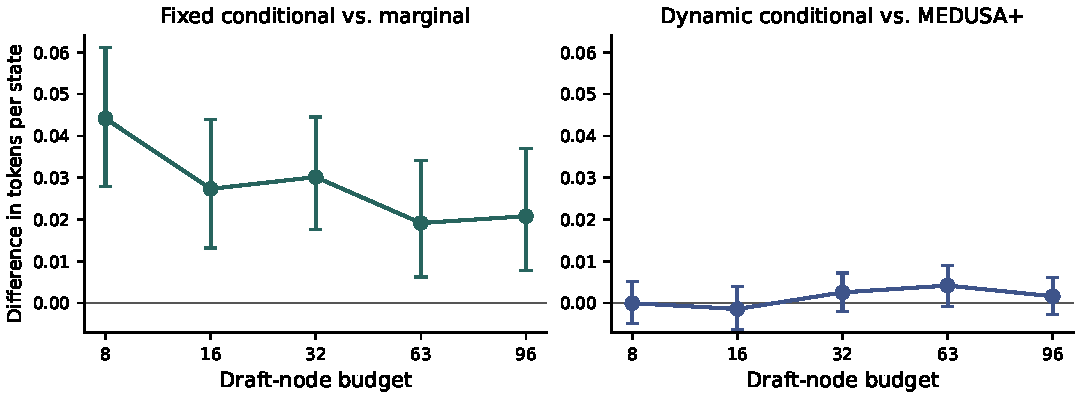
\includegraphics[width=.94\linewidth]{tables/paired_acceptance.pdf}
\caption{Change in accepted tokens per reference state at equal draft budgets. Bars show per-budget 95\% paired prompt-bootstrap intervals. Both panels use the same vertical scale.}
\end{figure}

\textbf{Validation and feature ablation.} Validation selected count smoothing $\alpha=3$, logistic inverse regularization $C=0.1$ and rank cap 4. Enlarging the direct classifier's training pool and adding its own selected nodes did not displace the original 64-node MEDUSA+ pool under the validation selection rule. The conditional logistic model's validation edge Brier score was 0.04566. Removing its confidence features raised the score to 0.04795, the largest change among the seven single-group ablations. Removing the uncertainty features raised it to 0.04597. These are conditional edge scores among accepted parents. The path scores in the main comparison apply to whole prefixes.

\textbf{Path calibration.} On 256,000 evaluation candidate nodes, 2.71\% matched the reference continuation. MEDUSA+ had the lowest Brier score (0.01839). Dynamic conditional regression had the lowest binned ECE (0.00125). Conditional counting improved on the fixed marginal model in both Brier and ECE. Small differences in average probability error need not alter which nodes enter the tree.


\subsection{Live verification and throughput}
\textbf{Reproducing historical precision failures.} The archived Colab run passed its strict check on 15 of 20 pilot prompts and 6 of 7 known cases. The two original detailed JSON reports were unavailable. On the laptop, all seven known cases passed, covering 855 observed rounds of static Medusa and dynamic MEDUSA+ across five budgets. We also reran the five historical pilot failures. Four passed. One of 818 observed rounds across those five prompts failed full-rank equality. At generation offset 19 under $B=32$, the tenth-ranked token of head five changed from ID 310 to 2821. That rank was unused by the selected tree. The largest absolute probability difference across ranked slots in that round was $1.61\times10^{-6}$. Cached and uncached greedy outputs, policy outputs, shared prefixes and selected-node labels all agreed on this subset. The trained head checksum matched the Colab archive. The GPU runtime differed. These observations locate the laptop disagreement. They cannot retrospectively assign a cause to the earlier failures.


On the trained-policy panel, all 80 policy--budget--prompt runs emitted the same token sequence as cached greedy, and every independently rerun greedy sequence matched its saved reference. Across 1,858 complete-horizon live rounds, 182 had at least one candidate-rank difference. Of 332 changed head/rank slots, 104 occurred at ranks used by the tree. Eight of 71,276 selected-node labels disagreed (0.011\%). All eight came from question 141 at generation offset 46 under $B=16$. The first head's sixth- and seventh-ranked tokens traded places for four policies. Each swap reversed one positive and one negative label, so the total number of matching selected nodes agreed in every observed round. These eight errors represent repeated observations of one state. Exact output agreement and agreement in accepted counts can coexist with errors in individual rank-path labels.


\textbf{Measured decoding speed.} The table gives generated tokens per second, throughput divided by cached greedy in the same budget run, and exact output matches out of eight measured questions. Higher throughput is better.
\begin{center}
\begin{tabular}{lrrrrrr}
\toprule
Policy & tok/s$_{16}$ & ratio$_{16}$ & exact & tok/s$_{63}$ & ratio$_{63}$ & exact\\
\midrule
Cached greedy & 9.92 & 1.000 & 8/8 & 10.64 & 1.000 & 8/8\\
Fixed marginal & 9.43 & 0.951 & 8/8 & 8.98 & 0.844 & 8/8\\
Fixed conditional & 9.31 & 0.939 & 8/8 & 8.64 & 0.812 & 8/8\\
MEDUSA+ & 9.60 & 0.968 & 8/8 & 8.85 & 0.832 & 8/8\\
Direct classifier & 9.52 & 0.959 & 8/8 & 8.33 & 0.783 & 8/8\\
Dynamic conditional & 9.40 & 0.947 & 8/8 & 8.26 & 0.776 & 8/8\\
\bottomrule
\end{tabular}
\end{center}


At $B=16$, MEDUSA+ was the fastest speculative policy at 9.60 tokens/s, versus 9.92 for greedy. At $B=63$, the fixed marginal tree led the speculative policies at 8.98 tokens/s, versus 10.64 for greedy. The gain in the fixed conditional tree's offline acceptance did not translate into higher throughput at either budget. On the timed $B=63$ panel, fixed marginal and fixed conditional committed 2.469 and 2.444 tokens per live round, respectively. Both the states visited and the set of prompts differ from full replay.

The separate profile of the first measured prompt at $B=63$ recorded 0.10 ms per round for the fixed conditional tree, 8.06 ms for MEDUSA+ and 20.42 ms for dynamic conditional scoring and buffer handling. At $B=16$ the corresponding values were 0.08, 2.57 and 6.90 ms. This overhead helps explain why the learned dynamic policy can be slower at similar acceptance. The two greedy baselines also differed, which is why each throughput ratio uses the baseline measured within its own budget run.


\section{Interpretation and limitations}
Conditioning helps the fixed tree where the independence approximation is most restrictive. A fixed marginal product uses the same rank accuracies on easy and difficult prefixes. Conditional counts change the order of paths that compete for a small number of nodes, including the all-top-rank path whose observed frequency exceeds its marginal-product prediction. The dynamic product already adapts to current head confidence. A logistic model can improve a calibration statistic while assigning essentially the same high-value nodes near the selection boundary. The small dynamic differences are consistent with that explanation. This experiment does not identify a unique cause.

The historical three-prompt replay suggested a larger fixed gain at $B=63$ ($+0.068$) and a negative dynamic difference ($-0.028$). The full evaluation yields smaller differences and changes the sign of the dynamic point estimate. The historical pilot used separately fitted models, teacher-forced features and a different runtime, so the comparison illustrates sensitivity to study design and sample size.

Three factors limit generalization. First, full-horizon replay omits generation tails and weights prompts according to their labeled length. Each live tree also visits a policy-dependent subset of states after committing multiple tokens. The observer checks labels on the branches actually selected online. Changed head probabilities or token ranks can still change which branches a replay policy would select. Second, the calibration pool emphasizes paths preferred by MEDUSA+, and Brier and ECE depend on that pool. Third, throughput depends on hardware and implementation. Fixed buffers are prepared before timing and dynamic trees use Python-side construction. The eight-question panel spans categories but provides only one measured question per category. Results concern greedy decoding on one frozen, quantized checkpoint at this generation cap.\par
\textbf{Reproducibility.} The accompanying repository contains the frozen prompt protocol, archive of token IDs and head ranks, fitted estimators and fixed trees, all 25 replay comparisons, per-prompt timing records and full numerical-verification reports \cite{code}. An independent token-level audit recovered all 89,410 training, validation and evaluation head labels exactly. The local project test suite passed all 87 tests.

\begin{thebibliography}{9}
\bibitem{medusa} T. Cai et al. Medusa: Simple LLM Inference Acceleration Framework with Multiple Decoding Heads. ICML, 2024. \url{https://proceedings.mlr.press/v235/cai24b.html}
\bibitem{plus} Z. Zhang. Acceleration Multiple Heads Decoding for LLM via Dynamic Tree Attention. 2025. \url{https://arxiv.org/abs/2502.05947}
\bibitem{direct} F. Huo et al. C2T: A Classifier-Based Tree Construction Method in Speculative Decoding. 2025. \url{https://arxiv.org/abs/2502.13652}
\bibitem{code} ECE 285 project repository. Trace contracts, prompt manifests, calibration and verification implementations. \url{https://github.com/alextung2/ECE_285_Final_Project}
\end{thebibliography}
\end{document}
